\begin{figure*}[t!]
    \centering
    
\includegraphics[width=1\linewidth]{Figure/framework.png}
    \caption{A holistic framework of GraphRAG and representative techniques for its key components.}
    \label{fig-frameworkGraphRAG}
\end{figure*}

\section{A Holistic Framework of GraphRAG}\label{sec-framework}
Based on existing literature on GraphRAG, we present a holistic framework of GraphRAG. Next, we introduce the basic problem setting and notation used throughout the whole framework.

\subsection{Problem Setting and Notations}
Following the general setting of RAG, given a graph-structured data source $G$, the user-defined query $Q$ is further sent to query processor $\boldsymbol{\Omega}^{\textbf{Processor}}$ to obtain the pre-processed query $\hat{Q}$. After that, the retriever $\boldsymbol{\Omega}^{\textbf{Retriever}}$ retrieves the content $C$ from the graph data source $G$ based on $\hat{Q}$. Next, the retrieved content $C$ is refined by the organizer $\boldsymbol{\Omega}^{\textbf{Organizer}}$ to formulate the refined content $\hat{C}$. Finally, the refined content $\hat{C}$ triggers the generator $\boldsymbol{\Omega}^{\textbf{Generator}}$ to generate the final answer $A$. The above five components are summarized as follows:


\begin{itemize}[leftmargin=*]
    \item \textbf{Query Processor $\boldsymbol{\Omega}^{\textbf{Processor}}$}: Preprocessing the given query $\hat{Q} = \boldsymbol{\Omega}^{\textbf{Processor}}(Q)$.

    \item \textbf{Graph Data Source $G$}: Information organized in graph-structured format.

    \item \textbf{Retriever $\boldsymbol{\Omega}^{\textbf{Retriever}}$}: Retrieve the content $C = \boldsymbol{\Omega}^{\textbf{Retriever}}(\hat{Q}, G)$ from $G$ based on the query $\hat{Q}$.

    \item \textbf{Organizer $\boldsymbol{\Omega}^{\textbf{Organizer}}$}: Arrange and refine the retrieved content $\hat{C}=\boldsymbol{\Omega}^{\textbf{Organizer}}(\hat{Q}, C)$. 

    \item \textbf{Generator}: Generate answers $A=\boldsymbol{\Omega}^{\textbf{Generator}}(\hat{Q}, \hat{C})$ to answer query $Q$.
\end{itemize}

Unlike sequential-based textual data and grid-structured image data, graph-structured data encapsulates relational information. To effectively harness this relational information, the above five core components of GraphRAG desire dedicated designs to handle graph-structured input/output and support graph-based operations. For example, in the retriever component, conventional RAG in the Natural Language Processing (NLP) utilizes sparse/dense encoders for index search~\cite{karpukhin2020dense, xiong2020answering}. In contrast, GraphRAG employs graph traversal methods (e.g., entity linking and BFS/DFS) and graph-based encoders (e.g., Graph Neural Networks (GNNs)) to produce embeddings for retrieval. 
This motivates us to summarize key innovations and representative designs of GraphRAG for each of the above five components under the holistic GraphRAG framework in the following.


\subsection{Task Applications and Example Query \texorpdfstring{$Q$}{Q}}
Similar to the general RAG framework where the text-formatted query $Q$ specifies the question context or the task instruction. Query $Q$ in GraphRAG could also be in the format of text. For example, in knowledge graph-based question-answering, the query could be "What is the Capital of China?"~\cite{luo2023reasoning, tian2024graph}. In addition, the query could also be in other formats, such as smile strings for molecular graphs~\cite{guo2023can}, or could even be the combination of multiple formats, such as the scene graph along with the text instruction~\cite{he2024g}. Table~\ref{tab-QA-summary} summarizes the common task applications and exemplary queries used in each domain, as well as their representative references.


% \begin{sidewaystable}
\begin{table*}[ht!]
    % \small
    \centering
    \caption{Summary of Task Applications and Exemplary Queries for GraphRAG in each domain.}
    \resizebox{\textwidth}{!}{
    % \renewcommand{\arraystretch}{0}
    \begin{adjustbox}{angle=90}
    \begin{tabular}{lp{4.5cm}p{15cm}p{7cm}
    }

    \toprule
    \textbf{Domain} & \textbf{Task Applications} & \textbf{Exemplary Query} & \textbf{References}\\
    \midrule

    %%%%%%%%%%%%%%%%%%%%%%%%%%%%
    \multirow{9}{*}{\textbf{\makecell[l]{Knowledge}}} 
    & \multirow{4}{*}{\textbf{\makecell[l]{KG QA}}} &  \multirow{4}{*}{\makecell[l]{Where is the 16th President of the United States?}} &  \cite{yasunaga2021qa,zhanggreaselm, yasunaga2022deep, sunthink, feng2020scalable, jiang2024hykge, delile2024graph, hu2022empowering, zhang2022subgraph, sanmartin2024kg, luo2023reasoning, knowledgenavigator, retrieve_rewrite_answer, wang2024reasoning, pullnet, pahuja2023retrieve, niu2024mitigating, tian2024graph, jiang2023structgpt, kim2024causal, gao2022graph, mvp_tuning, dai2024counter, luo2023chatkbqa, keqing, mavromatis2024gnn, gnn_llm, fang2024reano, wu2024stark, kim2023kg, wen2023mindmap, li2024dalk, unioqa, kgrank, li2024simple, wang2023knowledgpt, kgagent, zhu2024knowagent} \\    
    &  \textbf{KG Completion} & (Louvre, in, ?) & \cite{choudhary2023complex, pahuja2023retrieve, taunk2023grapeqa, kicgpt} \\
    & \textbf{Temporal QA} & Who was the president of the United States in 2006? & \cite{liao2024gentkg, gao2024two} \\
    & \textbf{Medical Prediction} & How long will the patient be spent in the hospital? & \cite{zhu2024emerge, zhu2024realm} \\
    & \textbf{Fact-Checking} & Who was the founder of Apple? & \cite{kim2023kg} \\
    & \textbf{Cyber Analysis and Defense} & Threat and vulnerability analysis & \cite{rahman2024retrieval} \\
    % & Entity Linking & \harry{todo} & \cite{} \\
    % & Relational Extraction & \harry{todo} & \cite{} \\
    %%%%%%%%%%%%%%%%%%%%%%%%%%%%
    \midrule
    %%%%%%%%%%%%%%%%%%%%%%%%%%%%
    \multirow{7}{*}{\textbf{\makecell[l]{Document}}} & \multirow{2}{*}{\textbf{\makecell[l]{Document Summarization}}} & \multirow{2}{*}{\makecell[l]{Please summarize the following documents.}} & \cite{yasunaga2017graph, wang2020heterogeneous, li2020leveraging, zhang2023contrastive, zhao2024hierarchical, xie2022gretel, zhang2023enhancing1, yang2018integrated, li2023compressed, chen2021sgsum, zhang2024coarse, edge2024local} \\ 
    & \textbf{Text Generation} & Please generate an abstract based on this paper and its references. & \cite{wang2024augmenting, chen2024llaga, kong2024gofa} \\ 
    & \textbf{Document Retrieval} & Find relevant documents related to Houston. & \cite{dong2024don, yu2021graph, zhang2018graph, liu2018matching, guo2024lightrag} \\
    & \textbf{Document Classification} &  What is the category of the following document?  & \cite{zhang2020every, liu2022hierarchical, zhang2020text, xiao2022graph} \\
    & \textbf{Document QA} & What are the main causes of climate change mentioned in the document? & \cite{nie2022capturing, wang2023docgraphlm, he2024g, wang2024knowledge, fang2019hierarchical}. \\
    & \textbf{Relational Extraction} & What is the relation between "Surfers Riverwalk" and "Queensland"? & \cite{wang2020global, nan2020reasoning, sahu2019inter, christopoulou2019connecting, zhou2020global, zhang2021improving} \\
    % & Node Classification &  &  \\
    % & Link Prediction &  &  \\
    %%%%%%%%%%%%%%%%%%%%%%%%%%%%
    \midrule
    %%%%%%%%%%%%%%%%%%%%%%%%%%%%
    \multirow{3}{*}{\textbf{\makecell[l]{Scientific}}} & \textbf{Molecule Generation} & Given an input molecule, retrieve exemplar molecules to guide the generation process. &\cite{wang2022retrieval, huanginteraction} \\
    & \textbf{Molecule Property Prediction} & Lumo is the lowest unoccupied molecular orbital energy. What's the Lumo value of this molecule? &\cite{liu2024moleculargpt} \\
    & \textbf{Scientific QA} & After meals, I feel a bit of stomach reflux. What medication should I take for it? & \cite{yang2024kg, jiang2024hykge, wen2023mindmap, li2024dalk, jeong2024improving,wu2024medical,delile2024graph,pelletier2024explainable,soman2024biomedical,wu2024medical} \\
    %%%%%%%%%%%%%%%%%%%%%%%%%%%%
    \midrule
    %%%%%%%%%%%%%%%%%%%%%%%%%%%%
    \multirow{5}{*}{\textbf{\makecell[l]{Social}}} & \textbf{Entity Property Prediction} & Morality Assessment, Partisanship Detection & \cite{jiang2023social, wang2024knowledge2} \\
    & \textbf{Text Generation} & Review Generation, Social Post Generation & \cite{ahmed2018learning, wang2024augmenting, kim2020retrieval, xie2023factual, sharma2018cyclegen, dong2017learning, park2015retrieval} \\
    & \textbf{Recommendation} & Graph-based/Sequential/Conversational Recommendation & \cite{du2024large, wei2024llmrec, wang2024knowledge2, huang2021graph, zeng2024federated, wang2023zero, qiu2020exploiting, hou2024large, friedman2023leveraging} \\
    & \textbf{Social QA} & What are the best parks for familiar gatherings around Los Gatoks? & \cite{zeng2024large, kemper2024retrieval, wu2024stark} \\
    & \textbf{Fake News Detection} & The COVID-19 vaccine contains microchips for government tracking. & \cite{ram2024credirag, li2024re} \\
    % & Node Classification &  &  \\
    % & Link Prediction &  &  \\
    %%%%%%%%%%%%%%%%%%%%%%%%%%%%
    \midrule
    %%%%%%%%%%%%%%%%%%%%%%%%%%%%
    \multirow{6}{*}{\textbf{\makecell[l]{Reasoning \\\& Planning}}} & \textbf{Sequential Plan Retrieval} & Please generate an image where a girl is reading a book, and her pose is the same as the boy in "example.jpg" & \cite{shen2024hugginggpt, shen2023taskbench, song2023restgpt, wu2024can, zhao2024large} \\
    & \textbf{Asynchronous Planning} & To make calzones, here are the steps and times required; please calculate the optimal plan for completion & \cite{lin2024graph} \\
    & \textbf{Commonsense Reasoning} & Infer the stance and generate/retrieve the corresponding commonsense explanation graph & \cite{saha2021explagraphs} \\
    % that explains the inferred stance
    & \textbf{Defeasible Inference} & Given a premise, a hypothesis may be weakened or overturned in light of new evidence & \cite{madaan2021could} \\
    & \textbf{Tool Usage} & Take Shower -> Walkto (bathroom) -> Walkto(shower) -> Find(shower) -> TurnTo(shower) & \cite{zhuang2023toolchain, hao2023reasoning} \\
    & \textbf{Embodied Planning} & Cook a potato and put it into the recycle bin & \cite{song2023llm, xu2024p} \\
    %%%%%%%%%%%%%%%%%%%%%%%%%%%%
    \midrule
    %%%%%%%%%%%%%%%%%%%%%%%%%%%%
    \multirow{8}{*}{\textbf{\makecell[l]{Tabular}}} & \textbf{Cell Type Prediction} &  What is the type of Cell B17? & \cite{jin2023tabprompt} \\
    & \textbf{Fraud Detection} & Is the following transaction legit or fraudulent? & \cite{rao2020xfraud,singh2023graphfc} \\
    & \textbf{Outlier Detection} & Is the data normal or anomalous? &\cite{goodge2022lunar,cheng2023anti, zhou2023detecting} \\
    & \textbf{CTR Prediction} & Given the history and advertisement features, predict the probability that a user will click on a specific ad. & \cite{li2019fi, du2022learning, guo2021dual} \\
    & \textbf{Data Imputation} & What is the missing value in cell B17 & \cite{zhong2023data, you2020handling, wu2021towards, cappuzzo2024relational}. \\
    & \textbf{Table Type Classification} & What is the category of the table? & \cite{wang2021tuta, jia2023getpt, jin2023tabprompt}. \\
    & \textbf{Table QA} & What is the average amount purchased and value purchased for the supplier who supplies the most products? & \cite{zhang2020cfgnn, zhang2020graph} \\
    & \textbf{Table Retrieval} & Retrieve tables containing information about the currencies of Asian countries & \cite{wang2021retrieving, cheng2021hitab} \\
    %%%%%%%%%%%%%%%%%%%%%%%%%%%%
    \midrule
    %%%%%%%%%%%%%%%%%%%%%%%%%%%%
    \multirow{1}{*}{\textbf{\makecell[l]{Infrastructure}}} & \textbf{Users Behavior Forecasting}  & pedestrians’ crossing actions;  lane change maneuvers & \cite{hussien2024rag} \\
    % Driver behavior forecasting &  & \cite{hussien2024rag} \\
    % & Edge Level Prediction &  & \cite{} \\
    % & Graph Level Prediction &  & \cite{} \\
    % & Utility Forecasting &  & \cite{} \\
    % & Vulnerability Analysis &  & \cite{} \\
    % & Reliability Analysis &  & \cite{} \\
    % & Resilience Analysis &  & \cite{} \\
    %%%%%%%%%%%%%%%%%%%%%%%%%%%%
    \midrule
    %%%%%%%%%%%%%%%%%%%%%%%%%%%%
    \multirow{2}{*}{\textbf{\makecell[l]{Scene}}} & \textbf{Visual QA} & Write a 500-word advertisement for this place in the scene graph that would make people want to visit it & \cite{he2024g} \\
    & \textbf{Embodied Planning} & Cook a potato and put it into the recycle bin & \cite{xu2024p} \\
    %%%%%%%%%%%%%%%%%%%%%%%%%%%%
    \midrule
    \multirow{5}{*}{\textbf{\makecell[l]{Biological}}} & \textbf{Gene Imputation} & What's the imputed gene value of the unsequenced gene KRAS for all cells?   & \cite{rao2021imputing, huang2020scgnn, wang2021scgnn, xu2021efficient, wen2022bi} \\
    %%%%%%%%%%%%%%%%%%%%%%%%%%%%
    & \textbf{Clustering} & What's the cluster for cell B17? & \cite{ciortan2022gnn, yu2022zinb, gan2022deep, cheng2022scgac} \\
    & \textbf{Multi-omics Prediction} & What's the protein expression provided by single-cell RNA-seq expression for cell B17? & \cite{wen2022graph} \\
    & \textbf{Cell Type Deconvolution} & What's the cell type proportion for spot A in the spatial transcriptomics data? & \cite{ding2024spatialctd, song2021dstg} \\
    & \textbf{Spatial Domain Identification} & What's the spatial domain for cell B17 in the spatial transcriptomics data? & \cite{hu2021spagcn, dong2022deciphering} \\
    %%%%%%%%%%%%%%%%%%%%%%%%%%%%
    \midrule
    %%%%%%%%%%%%%%%%%%%%%%%%%%%%
    \multirow{1}{*}{\textbf{\makecell[l]{Random}}} & \textbf{Graph Query} & What is the clustering coefficient of node P357 & \cite{fatemi2023talk, chai2023graphllm, bachmann2024pitfalls, dai2024revisiting, wang2024can, guo2023gpt4graph, luo2024graphinstruct} \\
    \bottomrule
    \end{tabular}
    \end{adjustbox}
    }

    \label{tab-QA-summary}
    
\end{table*}
% \end{sidewaystable}



\begin{figure*}[t!]
    \centering
    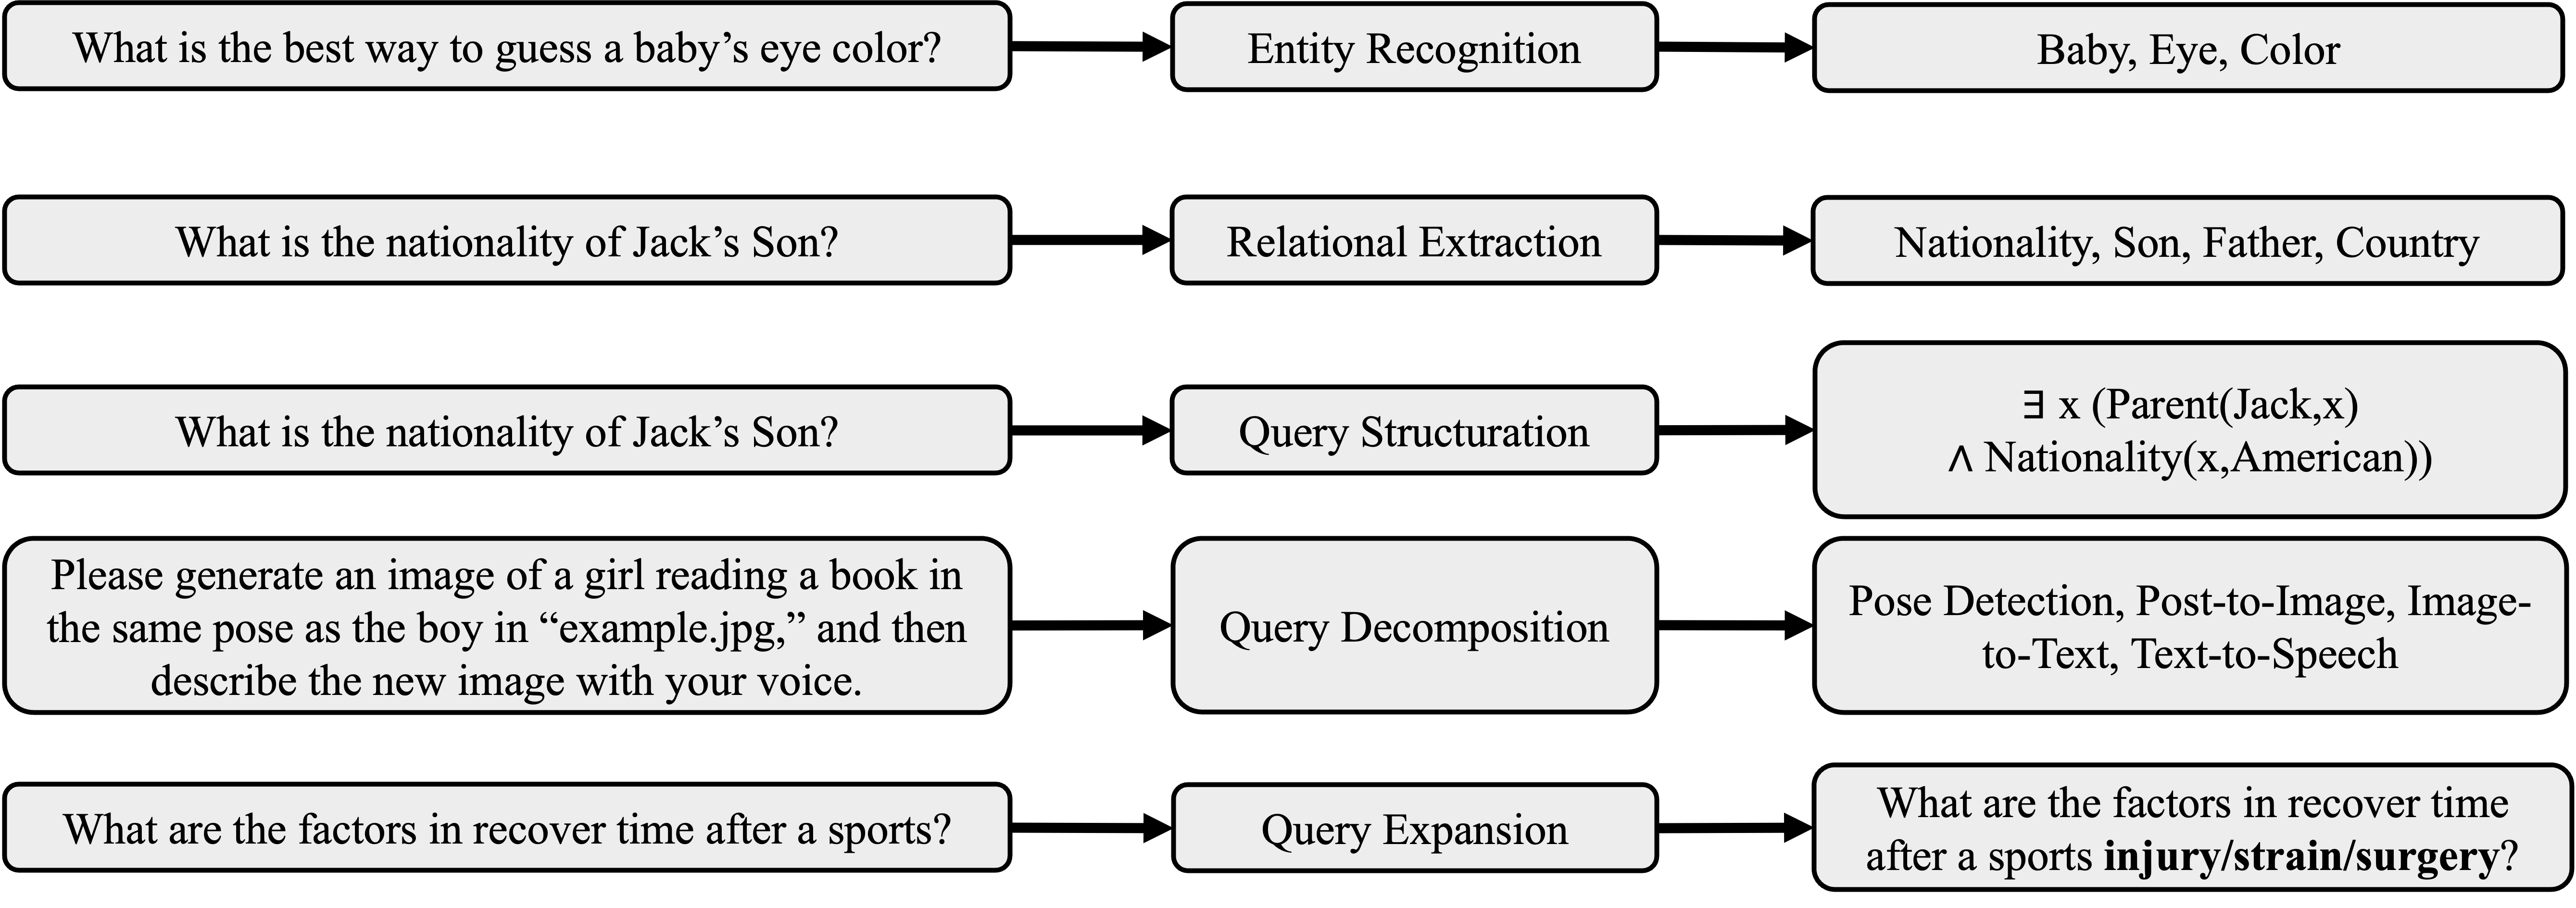
\includegraphics[width=1\linewidth]{Figure/query_tech.png}
    \caption{Existing techniques of query processor $\boldsymbol{\Omega}^{\text{Processor}}$ in GraphRAG.}
    \label{fig-query-process}
\end{figure*}


\begin{table}[t!]
\caption{Difference of query processor $\boldsymbol{\Omega}^{\text{Processor}}$ between RAG and GraphRAG.}
\resizebox{\linewidth}{!}{
\begin{tabular}{lcc}
\hline
\textbf{Technique} & \textbf{RAG} & \textbf{GraphRAG} \\
\hline
Entity Recognition & Extracting mentions in knowledge bases & Extracting mentioned nodes in graphs. \\
Relational Extraction & Extracting textual relations  & Extracting graph edge relations\\
Query Structuration & Structuring text query to SQL, SPARQL & Structuring text query to GQL  \\
Query Decomposition & Decomposed queries are separate  & Decomposed queries are logically related \\
Query Expansion & Expansion based on semantic knowledge & Expansion based on relational knowledge\\
\hline
\end{tabular}
}
\label{tab-query-process}
\end{table}

\newpage
\subsection{Query Processor \texorpdfstring{$\boldsymbol{\Omega}^{\text{Processor}}$}{Omega Processor}}

Unlike RAG, where both queries and data sources are purely text-formatted, data sources used in GraphRAG are graph-structured, which raises challenges in bridging text-formatted queries and graph-structured data sources. For example, the information that connects the knowledge graph and the query "Who is Justin Bieber's brother?" is not a specific passage but instead the entity "Justin Bieber" and the relation "brother of". Many techniques are proposed to correctly extract this information from the query, including entity recognition, relational extraction, query structuration, query decomposition, and query expansion. In the following, we first review each of these five query processing techniques within the broader NLP domain, followed by a focused examination of their unique adaptations for GraphRAG.


\subsubsection{Name Entity Recognition} \label{sec-ner}
Named Entity Recognition (NER) aims to identify mentions of entities from the text that belong to predefined categories, such as persons, locations, or organizations, and it serves as a fundamental component for numerous natural language applications~\cite{huang2021few, keraghel2024survey, li2020survey, meng2021distantly}. NER techniques can be broadly categorized into four main approaches: (1) rule-based methods, which rely entirely on handcrafted rules and require no annotated data; (2) unsupervised learning methods, which use unsupervised algorithms without labeled training examples; (3) feature-based supervised learning methods, which depend on supervised algorithms and careful feature engineering; and (4) deep learning approaches, which automatically discover representations needed after (un)-supervised training the deep learning models. Recent LLMs fall into the category of deep learning approaches and have demonstrated unprecedented success for NER. More details about these techniques and their resources can be found in~\citet{li2020survey}. 

Specifically, in the GraphRAG context, entity recognition primarily uses deep learning techniques (e.g., EntityLinker~\cite{tian2024graph, yasunaga2022deep} and LLM-based extraction~\cite{jin2024graph}) to identify entities in queries grounded by nodes in the given graph data sources. This step is vital for applications such as knowledge graph-based question answering~\cite{tian2024graph, yasunaga2021qa, yasunaga2022deep}. For example, given the question, "What is the best way to guess the color of the eye of the baby?", NER extracts entities such as "baby", "eye", and "color", which correspond to nodes in the knowledge graph and are treated as the seed nodes to initialize the retrieval process thereafter~\cite{wen2023mindmap, sanmartin2024kg}. For more recent GraphRAG research, NER has evolved beyond identifying the entity names but instead their structures. For example, \citet{jin2024graph} leverages LLMs to recognize node types in the graph, which further guides the retriever to identify nodes that match the recognized types for next-round exploration. For example, given the question "Who are the authors of `Language Models are Unsupervised Multi-task Learners'?" the initially recognized entity should not only be based on the semantic name "Language Models are Unsupervised Multi-task Learners" but also be based on the type of that entity, which is the paper node in this case. Accurately recognizing the names and structures of entities in GraphRAG reduces cascading errors and provides a solid foundation for subsequent retrieval and generation steps. 



\subsubsection{Relational Extraction}
Similar to NER, relational extraction (RE) is a long-standing technique in NLP to identify relations among entities and is widely applied to structured search, sentiment analysis, question answering, summarization, and knowledge graph construction~\cite{chen2018knowedu, li2020real, nasar2021named}. Recent advances in RE have been largely driven by deep learning techniques, and they can be summarized into three perspectives: text representation, context encoding, and triplet prediction, more details of which can be found in \citet{pawar2017relation, nasar2021named, han2020more}. 

For GraphRAG, RE serves two key purposes: constructing graph-structured data sources (e.g., knowledge graphs) by extracting triplets and matching the relations mentioned in the query and the graph data source to guide the graph search. For instance, given a query like "What is the capital of China?", relational extraction identifies the relation "capital of" and searches for corresponding edges via vector similarity in the knowledge graph, which guides the neighborhood selection and graph traversal direction~\cite{gao2024two, kim2023kg, luo2023reasoning, luo2024graph}. 



\subsubsection{Query Structuration}

Query structuration transforms queries into formats tailored to specific data sources and tasks. It often converts natural language queries into structured formats like SQL or SPARQL~\cite{jiang2023structgpt, li2023chain} to interact with relational databases. Recent advancements leverage pre-trained and fine-tuned LLMs to generate structured queries from natural language input to query databases. For graph-structured data, Graph Query Language (GQL) has emerged, such as Cypher, GraphQL, and SPARQL, which enables complex interactions with property graph databases. Additionally, \citet{jin2024graph} introduced a technique that decomposes complex queries into multiple structured operations, including node retrieval, feature fetching, neighbor checks, and degree assessment, enhancing precision and adaptability in querying.



\subsubsection{Query Decomposition}
Query decomposition~\cite{wong1976decomposition} aims to split the input query into multiple distinct subqueries, which are used to first retrieve sub-results and aggregate these sub-results together for the final results. In most existing RAG and GraphRAG, decomposed queries usually possess explicit logic connections that can handle complex tasks that require multistep reasoning and planning~\cite{lin2024graph, park2023graph, shen2023taskbench, song2023restgpt, xu2024p}. For example, a query like "Please generate an image where a girl is reading a book, and her pose is the same as the boy in `example.jpg' then describe the new image with your voice" involves multiple subtasks~\cite{xu2024p}, each of which would be completed by a specific sub-query. In addition, \citet{park2023graph} enhance the decomposition of the query by building a question graph where each sub-query is represented as a triplet within the graph. These graph-structured sub-queries effectively guide the retriever/generator through multi-step promptings.



\subsubsection{Query Expansion}
Query Expansion enriches a query by adding meaningful terms with similar significance~\cite{azad2019query}, which primarily addresses three challenges: (1) user-submitted queries are ambiguous and relate to multiple topics; (2) queries may be too brief to fully capture user intent; and (3) users are often uncertain about what they are seeking. Generally, it can be categorized into manual query expansion, automatic query expansion, and interactive query expansion. More recently, LLM-based query expansion has been a prominent area due to the creativity of the generated content\cite{chen2024analyze, jagerman2023query, lei2024corpus}

Unlike existing methods that mostly focus on textual similarities and overlook relations, QE in GraphRAG augments LLM expansion with structured relations. For example \citet{xia2024knowledge} expands the query by leveraging neighboring nodes of the mentioned entities in the query. Alternatively, \citet{keqing} convert the query into several sub-queries using pre-defined templates.


\subsection{Retriever \texorpdfstring{$\boldsymbol{\Omega}^{\textbf{Retriever}}$}{Omega Retriever}}
\label{sec:retriver}


After obtaining the processed query $\hat{Q}$, the retriever $\boldsymbol{\Omega}^{\textbf{Retriever}}$ identifies and retrieves relevant content $C$ from external graph sources $G$ to augment the downstream task execution:
\begin{equation}
    C = \boldsymbol{\Omega}^{\textbf{Retriever}}(\hat{Q}, G)
\end{equation}

Recently, retrievers have been increasingly integrated with LLMs to mitigate hallucination issues~\cite{tonmoy2024comprehensive}, address privacy concerns~\cite{zeng2024good}, and enhance explainability and dynamic adaptability~\cite{shi2024retrieval, wang2023knowledge}. While effective, they are predominantly designed for texts and images and not readily transferable to graph-structured data for GraphRAG for two reasons. First, the input/output format of GraphRAG differs significantly from that of traditional RAG. While most retrievers in RAG use NLP tokenizers for encoders and adhere to the "Text-in, Text-out" workflow, the workflow of GraphRAG is more diverse, including "Text-in, Text-out"~\cite{tian2024graph, wang2024knowledge}, "Text-in, Graph-out"~\cite{wu2024can, zhuangtoolchain}, "Graph-in, Text-out" and "Graph-in, Graph-out" processes~\cite{wangretrieval}. Secondly, retrievers in traditional RAGs do not capture graph structure signals. Methods like BM25 and TF-IDF~\cite{robertson2004simple, ramos2003using} primarily focus on lexical signals, and deep-learning-based retrievers~\cite  {karpukhin2020dense} usually capture semantic signals, both of which overlook the graph structure signals. This motivates us to review existing GraphRAG retrievers, i.e., heuristic-based, learning-based, and domain-specific retrievers, with a particular emphasis on their unique technical design adapted to graph-structured data.


\begin{figure*}[t!]
    \centering
    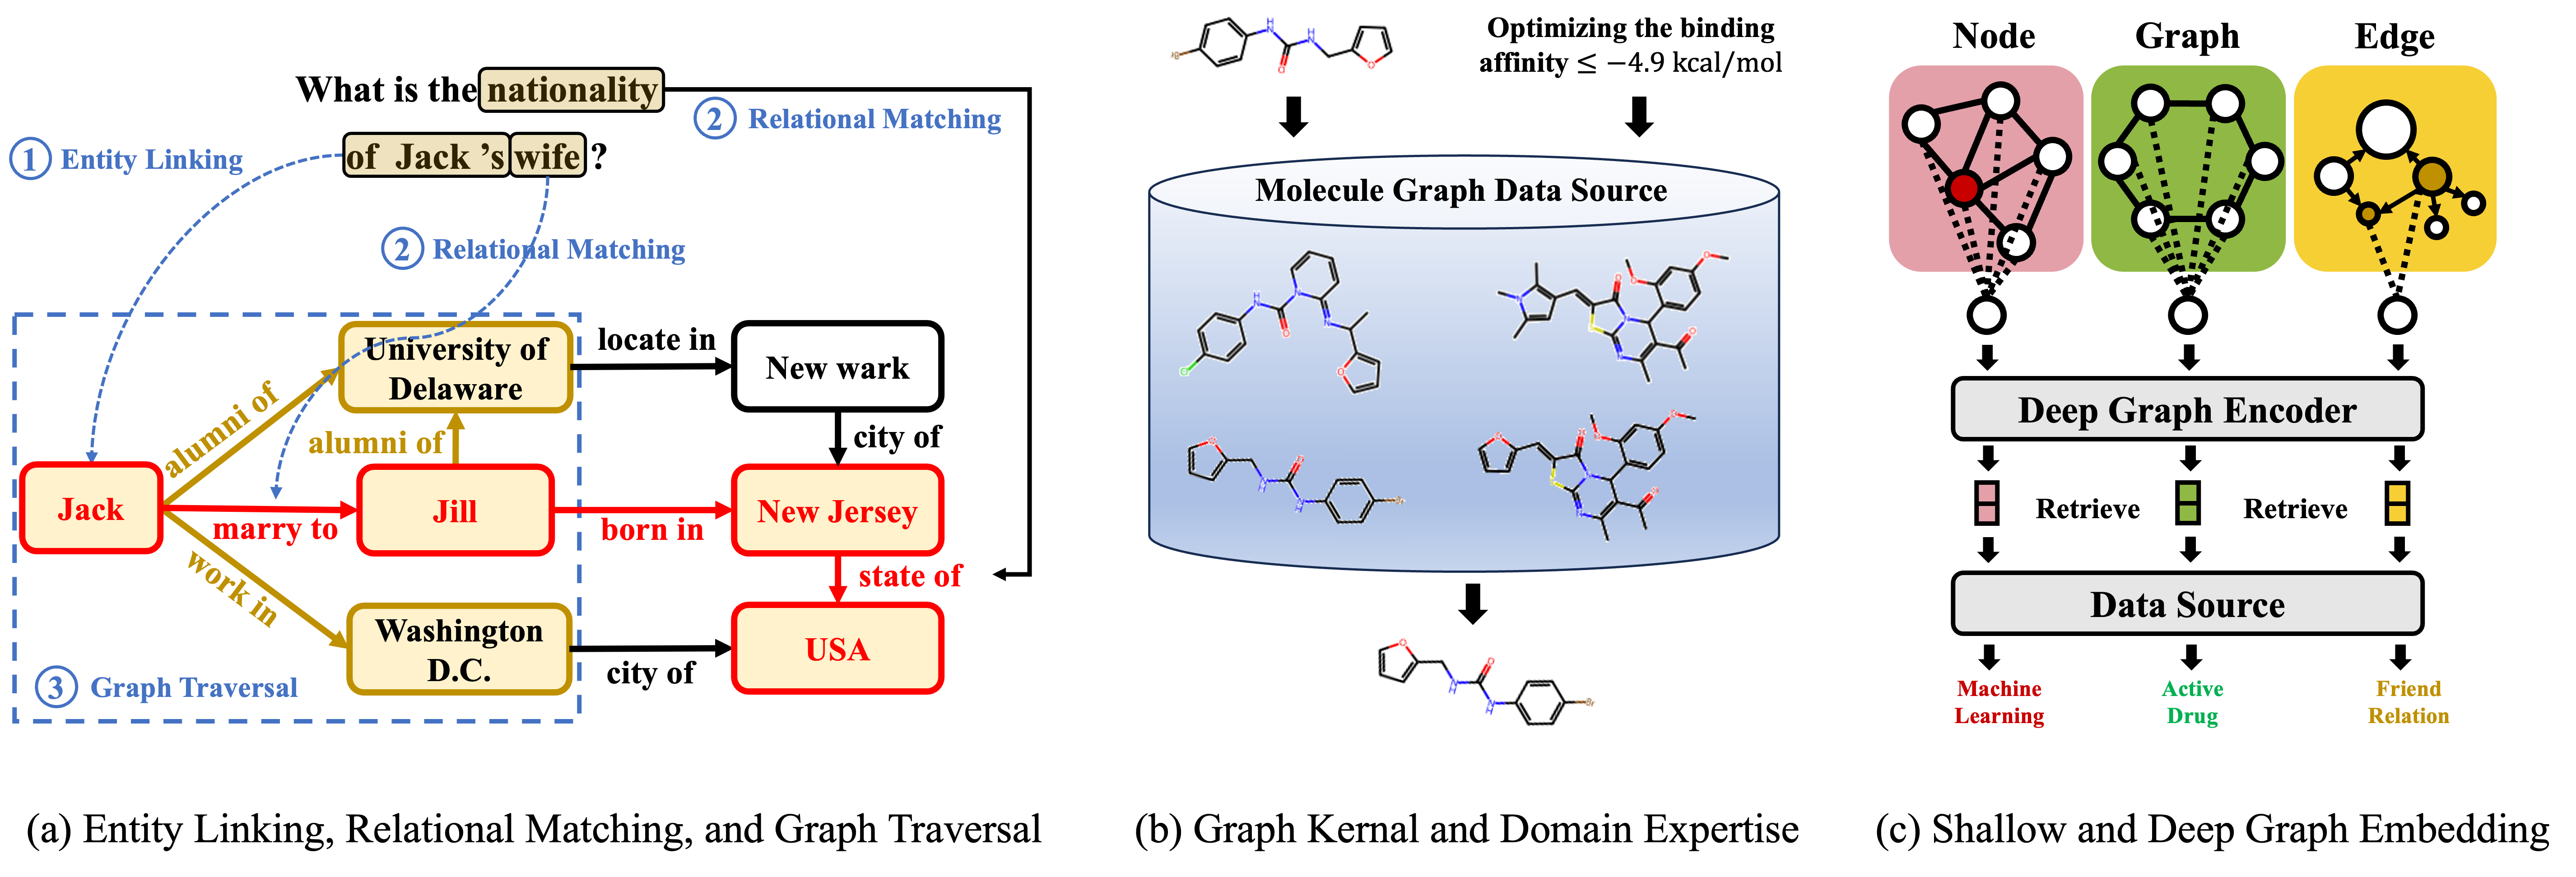
\includegraphics[width=1\linewidth]{Figure/retrieve_tech.png}
    \caption{Visualizing representative retrievers used in GraphRAG.}
    \label{fig-retriever-tech}
\end{figure*}


\begin{table}[t!]
\caption{Categorizing representative retrievers used in GraphRAG.}
\resizebox{\linewidth}{!}{
\begin{tabular}{lcccc}
\hline
\textbf{Method/Strategy} & \textbf{Input} & \textbf{Output} & \textbf{Description} \\
\hline
Entity Linking & Entity Mention & Node & Match query entity and graph node\\
Relational Matching & Relation Mention & Edge & Match query relation and graph edge \\
Graph Traversal & Node/Edge & Graph & Expand seed nodes/edges into subgraphs \\
Graph Kernel & (Sub)Graph & (Sub)Graph & Match query graph and candidate graph\\
\hline
Shallow Embedding & Any & Any & Embedding similarity match query and candidate\\
Deep Embedding & Any & Any & Embedding similarity match query and candidate\\
\hline
Domain Expertise & Expertise Rule & Any & Match Domain Expertise with nodes/edges/graphs\\
\hline
\end{tabular}
}
\label{tab-retriever}
\end{table}



\subsubsection{Heuristic-based Retriever}
Heuristic-based retrievers primarily use predefined rules, domain-specific insights, and hard-coded algorithms to extract relevant information from graph data sources. Their reliance on explicit rules often makes them more time/resource-efficient compared to deep learning models. For instance, simple graph traversal methods like BFS or DFS can be executed in linear time without needing training data. However, this same reliance on fixed heuristics also limits their adaptability to generalize to unseen scenarios. In the following, we review the heuristic-based retrievers commonly used in GraphRAG.


\textbf{Entity Linking}: In heuristic-based retrievers, entity linking involves mapping entities identified in the query to corresponding nodes in graph data sources. This mapping forms an initial bridge between the query and the graph, serving as either the retriever by itself or as a foundation for further graph traversal to broaden the scope of the retrieval. The effectiveness of this approach relies on accurate entity recognition conducted by the query processor and the quality of labeled entities on graph nodes. This technique is commonly applied in knowledge graphs, where Top-K nodes are selected as starting points based on their textual similarity to the query. The similarity metric can be computed using vector embeddings~\cite{wen2023mindmap, sanmartin2024kg} and lexical features~\cite{wang2024knowledge}. More recently, LLMs have been used as knowledgeable context augmenters to generate mention-centered descriptions as additional input to augment the long-tail entities where their limited training data usually cause the entity linking model to struggle to disambiguate~\cite{xin2024llmael}.


\textbf{Relational Matching}:
Relational matching, similar to entity linking, is a heuristic-based retrieval approach designed to identify edges within graph data sources that align with the relations specified in a query. This method is crucial for tasks that focus on identifying relationships among entities in a graph. The matched edges guide the traversal process by indicating which edges to explore next based on the entities and relations encountered in the graph data sources. Similar to entity linking, Top-K edges are selected based on their similarity to each edge in the graph~\cite{kim2023kg, gao2024two}.


In addition to the efficiency and simplicity of the above two types of heuristic-based retrievers, another key advantage is their ability to overcome ambiguity. For example, although machine/deep learning-based retrievers are difficult to differentiate semantically/lexically similar entities/relations (e.g., Byte vs. Bit, and President of vs. Resident of), these heuristic methods can easily distinguish them based on pre-defined rules, even in cases where semantic/lexical differences are subtle.


\textbf{Graph Traversal}:
After performing entity linking and relational matching to identify initial nodes and relations in graph data sources, graph traversal algorithms (e.g., BFS, DFS) can expand this set to uncover additional query-relevant information. However, a core challenge for traversal-based retrieval is the risk of information overload, as the exponentially expanding neighborhood often includes substantial irrelevant content. To address this, current traversal techniques integrate adaptive retrieval and filtering processes, selectively exploring the most relevant neighboring nodes and incrementally refining the retrieved content to minimize noise. This graph traversal is mainly used in GraphRAG for knowledge and document graphs. When traversing on these two types of graphs, many methods extract all paths less than length $l$ {\it between} the nodes identified by entity linking~\cite{yasunaga2021qa, yasunaga2022deep, zhanggreaselm, jiang2024hykge, feng2020scalable}, while others consider the $l$-hop subgraph around the initial entities~\cite{niu2024mitigating, tian2024graph, jiang2023structgpt, kim2024causal}. To more efficiently traverse the KG, other methods prune irrelevant paths via the use of a LLM~\cite{luoreasoning, sanmartin2024kg, wang2024knowledge, knowledgenavigator} and others use pre-defined rules or templates to traverse the graph~\cite{keqing, liao2024gentkg, dai2024counter}.

\textbf{Graph Kernel}:
Compared with the above heuristic-based retrievers for retrieving nodes, edges, and their combined subgraphs, some earlier works (e.g., graph extraction and image retrieval)~\cite{wu2016gksh, lebrun2008image, glavavs2013event} treat the text and image as the entire graph and use graph-level heuristics such as graph kernels to measure similarity and retrieve. Graph kernels measure pairwise similarities by calculating inner products between graphs, aligning both structural and semantic aspects of the query and the retrieved graphs. Notable examples include the random-walk kernel and the Weisfeiler Leman kernel~\cite{shervashidze2011weisfeiler, vishwanathan2010graph}. The random walk kernel computes similarity by performing simultaneous random walks on two graphs and counting the number of matching paths. The 
Weisfeiler Leman kernel iteratively applies the Weisfeiler Leman algorithm to produce color distributions of node labels at each iteration and then calculates similarity based on the inner products of these histogram vectors. For example, \citet{wu2016gksh} constructs event graphs of both documents and queries and uses a product graph kernel that counts walks between two graphs to measure the query-document similarity and rank the documents. \citet{lebrun2008image} conducts event graph matching by introducing a fast and efficient graph-matching kernel for image retrieval. Similarly, \citet{glavavs2013event} translates images into representative attribute structural graphs that capture spatial relations among regions and perform graph kernel based on random walks to derive hash codes for image retrieval. 



\textbf{Domain Expertise}:
The domain-agnostic nature of traditional heuristic-based methods restricts their effectiveness in areas that require specialized expertise. For instance, in drug discovery, chemists typically design drugs by referencing existing molecules with desirable properties rather than constructing molecular structures from scratch. These molecules are selected based on domain knowledge that guides the retrieval of structures with similar characteristics. Following this intuition, many GraphRAG systems incorporate domain expertise to enhance retriever design. \citet{wang2022retrieval} develop a hybrid retrieval system that integrates heuristic-based and learning-based retrieval to retrieve exemplar molecules that partially meet the target design criteria.


\subsubsection{Learning-based Retriever}
One significant limitation of heuristic-based retrievers is their over-reliance on pre-defined rules, which limits their generalizability to data that does not strictly adhere to these rules. For example, when confronted with entities that have slight semantic or structural variations, such as "doctor" and "physician", heuristic-based retrievers like entity linking may treat them differently due to their distinct lexical representations, despite their shared underlying meaning. To overcome this limitation, learning-based retrievers have been proposed to capture deeper, more abstract, and task-relevant relations between the query and objects in data sources, which avoid relying solely on hard-coded rules. These retrievers often work by uniformly compressing information of various formats (e.g., texts and images) into embeddings based on machine learning encoders and then fetching relevant information by conducting an embedding-based similarity search. Notably, some entity linking and relational matching methods that employ machine learning encoders to generate embeddings for matching should also be considered as learning-based retrievers. 

In conventional RAG, assuming the query $q$ and data sources that contain $n$ instances $S$ are embedded by corresponding encoders as $\mathbf{q} = \mathcal{F}_{q}(q) \in \mathbb{R}^{d}$ and $\mathbf{S} = \mathcal{F}_{S}(S) \in \mathbb{R}^{n\times d}$, we retrieve top-$k$ instances by similarity search according to the pre-defined similarity function $\phi$ in the embedding space. 
\begin{equation}
    \mathcal{S}^{*} = \argmax_{k}\phi(\mathbf{q}, \mathbf{S}),
\end{equation}

Unlike RAGs that use language and vision encoders to embed texts and images, encoders used in GraphRAG retrieval extend beyond independently and identically distributed (i.i.d.) data by embedding nodes, edges, and (sub)graphs. Depending on the input format, the encoder could be a text encoder for query, a graph-based encoder for graph structure, and an integrated text-and-graph encoder for the textual attributed graph~\cite{chen2023label, chen2024exploring}. We specifically focus on graph-based encoders. Existing graph-based encoders can be broadly categorized into shallow embedding methods -- such as Node2Vec and DeepWalk -- and deep embedding methods like Graph Neural Networks (GNNs). Below, we review these two encoders and their unique roles in GraphRAG. 


\textbf{Shallow Embedding Methods}:  
Shallow embedding methods~\cite{fey2019fast}, like Node2Vec~\cite{grover2016node2vec} and Role2Vec~\cite{ahmed2018learning}, learn node, edge, and graph embeddings that retain the essential structural information of the original graph. Based on the type of structural information that can be extracted, these methods generally fall into two categories: proximity/role-based embeddings. Proximity-based methods, such as DeepWalk and Node2Vec~\cite{grover2016node2vec, perozzi2014deepwalk}, focus on preserving the proximity of connected nodes, ensuring that nodes close in the graph also remain close in the embedding space. Role-based methods, like Role2Vec and GraphWave~\cite{ahmed2018learning, donnat2018learning}, generate node embeddings based on their structural roles rather than their proximity relations. In general, these methods initialize each node with a latent embedding vector and conduct unsupervised training to squeeze structural signals derived from graph structure into the embedding. In GraphRAG, proximity-based shallow embeddings can effectively retrieve entities that are proximally close, while role-based embeddings can capture entities that share similar roles. For instance, proximity-based embeddings could be used to retrieve academic papers by fetching papers sharing similar research topics or retrieve reviews from products that are co-purchased with the current product~\cite{salemi2023lamp, wang2024augmenting}. Meanwhile, role-based embeddings could support tasks like generating company emails by retrieving similar emails based on shared roles or tones~\cite{wang2024augmenting}.



\textbf{Deep Embedding Methods}:
Although shallow embedding methods incorporate structural signals into learned embeddings for nodes, edges, or entire graphs, they struggle to leverage semantic features—like bag-of-words representations for academic paper retrieval or atomic numbers for molecular retrieval~\cite{fey2019fast}. Additionally, these methods lack inductivity, requiring re-initialization and retraining whenever new nodes, edges, or graphs are added. This limitation significantly reduces their applicability in GraphRAG retrieval tasks as real-world knowledge evolves dynamically where new information continually replaces outdated content, such as in citation networks, social graphs, and knowledge graphs~\cite{cheng2024multi, wang2023knowledge, wu2024updating}. To address these limitations, deep embedding methods have been proposed, which not only jointly fuse features and graph structures to obtain embeddings for retrieval but also inherent inductive property as the newly coming nodes/edges/graphs share common feature space with the ones during the training phase. One of the most representative and powerful approaches in this category is GNN, which combines the power of message-passing to encode structural signals and feature transformation to extract task-relevant information. Mathematically, $l^{\text{th}}$-layer graph convolution can be formulated as:

\begin{align}
    \mathbf{x}_i^l &= \gamma_{\boldsymbol{\Theta}_{\gamma}} \left( \mathbf{x}_i^{l-1} \oplus \sum_{j \in \mathcal{N}_{i}} \phi_{\boldsymbol{\Theta}_{\phi}} \left( \mathbf{x}_i^{l-1}, \mathbf{x}_j^{l-1}, \mathbf{e}_{ij} \right) \right),~~~~~~~~~~~~~~~~~~\text{Node-level} \label{eq-node_level}\\
    \mathbf{e}_{ij}^l &= \gamma_{\boldsymbol{\Theta}_{\gamma}} \left( \mathbf{e}_{ij}^{l-1} \oplus \sum_{e_{mn} \in \mathcal{N}_{ij}^{e}} \phi_{\boldsymbol{\Theta}_{\phi}} \left( \mathbf{e}_{ij}^{l-1}, \mathbf{e}_{mn}^{l-1}, \mathbf{x}_{e_{ij}\cap e_{mn}} \right) \right),~~~~\text{Edge-level} \label{eq-edge_level}\\
    \mathbf{G}^l &= \rho_{\boldsymbol{\Theta}_{\rho_G}}(\{\mathbf{x}_i^l, \mathbf{e}_{ij}^l \mid v_i \in \mathcal{V}_G, e_{ij} \in \mathcal{E}_{G}\}),~~~~~~~~~~~~~~~~~~~~~~~~~~~~~~~\text{Graph-level} \label{eq-graph_level}
\end{align}


In node-level graph convolution, each node $v_i$ adaptively aggregates the embeddings of its neighboring nodes $\mathcal{N}_i$, with weights based on edge features via the weighting function $\phi_{\boldsymbol{\Theta}_{\phi}}$. The aggregated neighborhood embeddings are then combined with the node's own embedding from the previous layer $\mathbf{x}_i^{l-1}$, using a combination function $\gamma_{\boldsymbol{\Theta}_{\gamma}}$, as shown by Eq~\eqref{eq-node_level}. Optimizing loss from training downstream tasks would enable the weighting function $\phi_{\boldsymbol{\Theta}_{\phi}}$ to prioritize the most important neighbors and enable the combination function $\gamma_{\boldsymbol{\Theta}_{\gamma}}$ to balance contributions from the node’s neighborhood and its own embedding. Similarly, in edge-level graph convolution, the same aggregation principle applies, but the neighbors of an edge are edges incident to the same ending points of that edge $\mathcal{N}^e_{ij}$, as shown by Eq~\eqref{eq-edge_level}. Graph-level embeddings could be obtained by further applying pooling operation $\rho_{\boldsymbol{\Theta}_{\rho}}$ over node and edge embeddings, as shown by Eq~\eqref{eq-graph_level}. Following this GNN-based embedding paradigm, various forms of graph knowledge from diverse sources—such as nodes, edges, and (sub)graphs—can be uniformly embedded into vector representations, as shown in Figure~\ref{fig-retriever-tech}(c) where we derive embeddings for nodes ($\mathbf{X}$), edges ($\mathbf{E}$), and graphs ($\mathbf{G}$). 


Having obtained these node/edge/graph-level embeddings further enables us to create embeddings for different types of structures ($\mathbf{S}$) by combining these sub-structure embeddings according to specific configurations for each structure. For instance, if the retrieved subgraph is a path within a knowledge graph, we can aggregate the embeddings of the nodes and relations along that path to form a cohesive path embedding.\footnote{Incorporating structural signals may be necessary, a consideration to be addressed in future work.} Eventually, the resulting embeddings for different structures can be utilized either during the training phase to optimize query alignment or during the testing phase to enable similarity-based neural search. For example, GNN-RAG~\cite{sanmartin2024kg} uses a GNN to perform retrieval, where a separate round of message passing is performed for each query. The query $\hat{Q}$ is incorporated into the message passing by, including its embedding in the message computation. A set of ``candidate'' nodes is chosen which have a probability of being relevant greater than some threshold. The shortest path from the query nodes to each candidate node is retrieved as context. \citet{gnn_llm} consider the use of a conditional GNN~\cite{conditional_mpnn} where only the linked entities from the query are initialized to a non-zero representation. The candidate nodes are chosen in a similar manner to~\cite{sanmartin2024kg}. A single path is then retrieved for each candidate node and is extracted by backtracking until we reach a query node. REANO~\cite{fang2024reano} encodes the query information into an edge-specific attention weight, conditional on the query. After aggregation, the top k triples most similar to the query are chosen as context.



\subsubsection{Advanced Retrieval Strategies}
Real-world queries are often complex and encode multi-aspect intentions, possess structure patterns, and desire multi-hop reasoning that the aforementioned basic retrievers struggle to address. For example, answering "What is the name of the fight song of the university whose main campus is in Lawrence, Kansas, and whose branch campuses are in the Kansas City metropolitan area?" demands multi-hop reasoning to identify the university based on location and retrieve information about its fight song~\cite{he2024make, trivedi2022interleaving}. Similarly, a query like "What are the main themes in the dataset?" requires understanding the product community structure, retrieving themes for each community, and aggregating the identified themes together to summarize the main theme~\cite{edge2024local}. Furthermore, when asking "Who is the most impactful research scholar in deep learning?" the answer could vary depending on multiple aspects~\cite{zhang2023pre}, such as the number of citations, the volume of published papers, or the number of co-authors. Accurately addressing such queries requires a deeper understanding of the underlying data distribution to discern which aspect the query prioritizes. To address these highly complex queries, advanced retrieval strategies have been proposed, and we review them as follows:



\textbf{Integrated Retrieval:} Integrated retrieval combines various types of retrievers to capture relevant information by balancing their strengths and weaknesses. Typically, integrated retrieval approaches are categorized according to which individual retrievers are used in combination, with notable examples including neural-symbolic retrieval~\cite{dietz2023neuro, lee2024diakop, wang2024knowledge} and multimodal retrieval~\cite{cui2024more, long2024generative}. 

Since the knowledge stored in graph-structured data exists mostly in symbolic format, neural-symbolic retrieval is a natural choice for the integrated retrieval strategy in GraphRAG. This strategy interleaves rule-based patterns for retrieving symbolic knowledge with neural-based signals for retrieving more abstract and deep knowledge. For example, \citet{luo2023reasoning, wen2023mindmap} first expands the neighbors based on the knowledge of the symbolic knowledge graph and then performs path retrieval using neural matching. In contrast, \citet{mavromatis2024gnn} first utilizes GNNs to retrieve seed entities (neural retrieval) and then extract the shortest paths from seed entities (symbolic retrieval). Similarly, \citet{tian2024graph, yasunaga2021qa, yasunaga2022deep, wang2024knowledge2, luo2023reasoning} fetch the k-hop neighborhood of the entities mentioned in the current question-answering pair and the session of user-generated items as the answer candidates (symbolic retrieval) and compute attention between the query and the extracted subgraph to differentiate candidate relevance (neural retrieval).


\textbf{Iterative Retrieval:} Iterative retrieval is a multistep process where consecutive retrieval operations share common dependencies such as causal, resource, and temporal dependency. These dependencies can be implicitly characterized by the retrieval order in RAG~\cite{trivedi2022interleaving, yang2024rag} or explicitly modeled as a graph structure in GraphRAG~\cite{he2024make, wu2024can}. Consequently, iterative retrieval is primarily utilized in GraphRAG to capture these dependencies. For example, KGP~\cite{wang2023knowledge} alternates between generating the next piece of evidence for the question and selecting the most promising neighbor. ToG~\cite{sunthink} starts by identifying initial entities and then iteratively expands reasoning paths until enough information is gathered to answer the question. StructGPT~\cite{jiang2023structgpt} pre-defines graph interfaces and prompts LLMs to iteratively invoke these interfaces until sufficient information is collected. 


\textbf{Adaptive Retrieval:} While retrieved external knowledge offers benefits, it also introduces risks. If the generator already possesses sufficient internal knowledge for a task, the retrieved external information may be unnecessary or even conflicting~\cite{chen2022rich, xu2024knowledge}. Specifically, when internal knowledge fully covers the necessary information, retrieval becomes redundant and may introduce contradictions. To mitigate this, knowledge checking has been proposed in RAG systems~\cite{jeong2024adaptive, jin2024tug, wang2024astute, yao2024seakr}. This approach allows the system to adaptively assess when and how much external information is needed. By equipping the retriever with this adaptability, RAG can provide more intelligent, flexible, and context-aware responses, fostering better harmony between internal and external knowledge sources.

One of the adaptive retrievals in GraphRAG is designed by considering different reasoning depths for different queries, i.e., too few hops of graph traversal might overlook critical reasoning relations, while too many can introduce unnecessary noise. \citet{knowledgenavigator, wu2023retrieve} address this by training models to predict the required number of hops for a given query and retrieving the relevant graph content accordingly. No existing works focus on resolving knowledge conflicts in GraphRAG, and therefore, we leave this discussion to future work.

\subsection{Organizer}\label{sec:organizer}
After retrieving the relevant content $C$ from external graph data sources, which may be in the format of entities, relations, triplets, paths or subgraphs, the organizer $\boldsymbol{\Omega}^{\textbf{Organizer}}$ processes this content in conjunction with the processed query $\hat{Q}$. The aim is to post-process and refine the retrieved content to better adapt it for generator consumption, thereby further improving the quality of the downstream content generation. Formally, the organizer is represented as follows:
\begin{align}
    \hat{C} = \boldsymbol{\Omega}^{\textbf{Organizer}}(\hat{Q}, C)
\end{align}

In GraphRAG, the need for fine-grained organization and refinement of retrieved content is driven by several key reasons. Firstly, when the retrieved contents are subgraphs, their heterogeneous format of knowledge in terms of node/edge features and graph structures becomes more likely to include irrelevant and noisy information, which poses significant difficulty for LLM to digest and thus compromises the generation quality. This raises the desire for graph pruning techniques to polish the retrieved subgraph and remove task-irrelevant knowledge. Secondly, LLMs have been widely demonstrated to possess attention biases toward certain positions of relevant information within the retrieved context~\cite{chen2023understanding}. Therefore, the exponentially growing neighbors as the receptive field enlarges (i.e., the number of hops increases) in the retrieved subgraphs would also exponentially increase the amount of context length in the prompt and dilute the focus of LLMs on the task-relevant knowledge~\cite{shi2023large}. This poses a new requirement for the graph-based reranking mechanism to prioritize the most important content within the retrieved graph. Thirdly, the retrieved content might be incomplete in terms of both the semantic content and the structural content, which necessitates graph augmentation for the enhancement. Finally, the retrieved content is often a graph, which not only possesses semantic content information but also owns its unique structure. This complex structural content is not easily consumed by LLMs that are trained by next-token prediction coupled with linearized prompting, which requires structure-aware verbalization techniques to reorganize. We will formally review each of the above-motivated organizer techniques in the following sections.



\subsubsection{Graph Pruning}
In GraphRAG, the retrieved graph can be large and potentially contain a significant amount of noisy and redundant information. For example, when graph traversal methods are applied in retrieval, the size of the retrieved subgraph exponentially increases with the number of hops. Large subgraph sizes not only increase computational costs but can also reduce generation quality due to the inclusion of noisy information. In contrast, if the number of hops is too small, the retrieved subgraph may be too small to include crucial knowledge required by tasks. To achieve a better trade-off between the size of the retrieved subgraph and the amount of its encoded task-relevant information, various graph pruning methods have been proposed to reduce the size of subgraphs by removing irrelevant nodes and edges while preserving the essential information.

\begin{itemize}[leftmargin=*]
    \item \textbf{Semantic-based pruning:}  Semantic-based pruning focuses on reducing the graph size by removing nodes and edge relations that are semantically irrelevant to the query. For example, QA-GNN~\cite{yasunaga2021qa} prunes irrelevant nodes with low relevance scores by encoding the query context and node labels using LLMs, followed by a linear projection. GraphQA~\cite{taunk2023grapeqa} further removes clusters of nodes with the lowest relevance to the query. KnowledgeNavigator~\cite{guo2024knowledgenavigator} scores the relations in the retrieved graph based on the query and prunes irrelevant relations to reduce graph size. Additionally, \citet{gao2022graph} partition the retrieved subgraph into smaller subgraphs and then ranks them with only the top-k smaller subgraphs retained for generations. G-Retriever~\cite{he2024g} defines a semantic score for each retrieved node and edge, then refines the graph by solving the prize-collecting Steiner tree problem to construct a more compact and relevant subgraph.
    \item \textbf{Syntactic-based pruning:} Syntactic-based pruning removes irrelevant nodes from a syntactic perspective. For instance, \citet{su2024pipenet} leverages dependency analysis to generate a parsing tree of the context and then filters the retrieved nodes based on their span distance from the parsing tree.
    \item \textbf{Structure-based pruning:} Structure-based pruning methods focus on pruning the retrieved graph based on its structural properties. For example, RoK~\cite{wang2024reasoning} filters out reasoning paths in the subgraph by calculating the average PageRank score for each path. Other works, such as \citet{jiang2023structgpt} and \citet{he2021improving}, also leverage PageRank to extract the most relevant entities.
    \item \textbf{Dynamic pruning:} Unlike the aforementioned methods, which typically prune the graph once, dynamic pruning removes noisy nodes dynamically during training.  For example, JointLK~\cite{sun2021jointlk} uses attention weights to recursively remove irrelevant nodes at each layer, keeping only a fixed ratio of nodes. Similarly, DHLK~\cite{wang2023dynamic} filters out nodes with attention scores below a certain threshold dynamically during the learning process.
\end{itemize}

\subsubsection{Reranker}

The performance of LLMs can be influenced by the position of relevant information within the context, whether it appears at the beginning, middle, or end~\cite{chen2023understanding}. Additionally, LLMs' generation is impacted by the order in which in-context knowledge is provided, with later documents contributing less than earlier ones~\cite{ivgi2023efficient, liu2024lost}. While retrieved information is typically ordered by relevance scores during the retrieval process, these scores are often based on coarse-grained rankings across a large set of candidates. Enhancing reordering solely among the retrieved information at a fine-grained level, a process known as re-ranking, is essential to achieve optimal downstream performance. For example, \citet{li2023graph} rerank retrieved triples using a pre-trained cross-encoder. \citet{jiang2024hykge} and \citet{liu2024knowledge} employ pre-trained reranker models to rerank retrieved paths. \citet{yu2021kg} train a GNN to rerank the retrieved passages.  \citet{liao2024gentkg} order the paths by the time they occurred, giving more emphasis to recent paths. 

\subsubsection{Graph Augmentation}
Graph augmentation aims to enrich the retrieved graph to either enhance the content or improve the robustness of the generator. This process can involve adding supplementary information to the retrieved graph, sourced from external data or knowledge embedded within LLMs.  There are two main categories of methods:
\begin{itemize}[leftmargin=*]
    \item \textbf{Graph Structure Augmentation:} Graph structure augmentation methods involve adding new nodes and edges to the retrieved graph. For instance, GraphQA~\cite{taunk2023grapeqa} augments the retrieved subgraph by incorporating noun phrase chunk nodes extracted from the context. Moreover, \citet{yasunaga2021qa} and \citet{taunk2023grapeqa} treat the query as a node, integrating it into the retrieved graph to create direct connections between the query and relevant information. \citet{tang2024cross} augment the graph structure based on pretrained diffusion models. 
    \item \textbf{Graph Feature Augmentation:} Graph feature augmentation methods focus on enriching the features of the nodes and edges in the graph. Since the original features might be lengthy or sparse, data augmenters can be employed to summarize or provide additional details for these features. For example, Once~\cite{liu2024once} uses LLMs as Content Summarizers, User Profilers, and Personalized Content Generators in recommendation systems. Similarly, LLM-Rec~\cite{lyu2023llm} and KAR~\cite{xi2024towards} apply various prompting techniques to enrich node features, making them more informative for downstream tasks.
\end{itemize}

Additionally, some graph augmentation techniques focus solely on the retrieved graph itself, such as randomly dropping nodes, edges, or features to improve model robustness. \citet{ding2022data} provide a systematic review of these data augmentation methods.


\subsubsection{Verbalizing}
\label{sec:verbalizing}
Verbalizing refers to converting retrieved triples, paths or graphs into natural language that can be consumed by LLMs. There are two main approaches to verbalization: linear verbalization and model-based verbalization.

Linear verbalization methods typically convert graphs into text using predefined rules. The primary techniques for linear verbalization include:

\begin{itemize}[leftmargin=*]
    \item \textbf{Tuple-based:} These methods place the different pieces of retrieved information and order them in a tuple~\cite{baek2023knowledge, oguz2020unik}. For example, when performing retrieval on a KG, many methods retrieve a set of facts. A single fact is verbalized in the generation prompt as the tuple $(\text{entity} \: 1, \text{relation} \: 1, \text{entity} \: 2)$~\cite{niu2024mitigating,  tian2024graph}. For a set of facts, we first sort them in a specific order, and then verbalize them one at a time as an individual tuple. Each piece of information is typically separated by line in the prompt. Note that the same logic can be applied to paths, nodes, and so on.


    \item \textbf{Template-based:} These methods verbalize paths or graphs using predefined templates to generate more natural text. For example, LLaGA~\cite{chen2024llaga} proposes some templates such as Hop-Field Overview Template to convert graph into sequence. For KGs, several methods~\cite{knowledgenavigator, unioqa} convert individual facts into natural text. For example, \citet{knowledgenavigator} convert a fact (entity 1, relation, entity 2) to text using the template {\it ``The \{relation\} of \{entity 1\} is/are: \{entity 2\}''}.
\end{itemize}

Model-based verbalization methods typically use fine-tuned models or LLMs to convert input facts into coherent and natural language. These methods generally fall into two categories:

\begin{itemize}[leftmargin=*]
    \item \textbf{Graph-to-text verbalization}: These methods focus on converting retrieved graphs into natural language while preserving all the information. For instance, \citet{koncel2019text} and \citet{wang2020amr} leverage graph transformers to generate text from knowledge graph. \citet{ribeiro2020investigating} evaluate several pretrained language models for graph-to-text generation, while \citet{wu2023retrieve}, and \citet{agarwal2020knowledge} fine-tune LLMs to transform graphs into sentences, ensuring a faithful representation of the graph content in textual form. 
    
    \item \textbf{Graph Summarization:}  In contrast to Graph-to-Text Verbalization, which retains all details, Graph Summarization methods aim to generate concise summaries based on the retrieved graph and the query. EFSum~\cite{ko2024evidence} proposes two approaches: one directly prompts LLMs to summarize the retrieved facts and query, while the other fine-tunes LLMs specifically for summarization tasks. CoTKR~\cite{wu2024cotkr}, on the other hand, alternates between two operations: Reasoning, where it decomposes the question, generates a reasoning trace, and identifies the specific knowledge needed for the current step; and Summarization, where it summarizes the relevant knowledge from the subgraph that retrieved based on the current reasoning trace.
\end{itemize}


\subsection{Generator}
\label{sec:generator}

The generator aims to produce the desired output for specific tasks based on the query and the retrieved information. These tasks can range from discrimination tasks (e.g., node/edge/graph classification) to generation tasks (e.g., KG-based question answering) and graph generation (e.g., molecular generation). Due to the uniqueness of different tasks, different generators are often desired. We categorize generators into three main types:  Discriminative-based Generators, which leverage models like GNNs and Graph Transformers for tasks like classification; LLM-based Generators, which utilize the capabilities of LLMs to generate answers for text-based tasks; and Graph-based Generators, which generate new graphs using generative models such as diffusion models. Next, we provide a detailed illustration of these generators.

\subsubsection{Discrimination-based Generator}
Discrimination-based generators focus on discriminative and regression tasks, which can typically be modeled as graph tasks, such as node, edge, or graph classification and regression. Models designed for graph data, such as GNNs and Graph Transformers, are widely used as discrimination-based generators. The choice of GNN depends on the graph type and task.  For instance, GCN~\cite{kipf2016semi}, GraphSAGE~\cite{hamilton2017inductive}, and GAT~\cite{velivckovic2017graph} are typically applied to homogeneous graphs, whereas models like RGCN~\cite{schlichtkrull2018modeling} and HAN~\cite{wang2019heterogeneous} are used for heterogeneous graphs, and HGNN~\cite{feng2019hypergraph} and Hyper-Attention~\cite{bai2021hypergraph} are suitable for hypergraphs. Additionally, graph transformers~\cite{min2022transformer, shehzad2024graph} have gained popularity for their ability to capture global dependencies.
Additionally, different training strategies, such as (semi-)supervised learning~\cite{ma2021deep} and graph contrastive learning~\cite{ju2024towards, liu2022graph}, are employed depending on the specific requirements of the task.

\subsubsection{LLM-based Generator}
LLMs have demonstrated remarkable capabilities in understanding and generating natural language across a wide range of tasks. However, LLMs are inherently designed to process sequential data, while the retrieved information in GraphRAG is typically structured as graphs. Although various GraphRAG organizers, such as verbalization methods, convert retrieved graph information into text, these transformations may result in the loss of important graph structure information, which could be crucial for certain tasks. To take advantage of the ability of LLMs, many research efforts have been proposed to feed the graph information into LLMs, and we summarize them into the following categories:

\begin{itemize}[leftmargin=*]
    \item \textbf{Verbalizing:} Verbalizing aims to convert the retrieved information in GraphRAG into sequences that can be processed by LLMs. These methods are detailed in Section~\ref{sec:verbalizing}. 

    \item \textbf{Embedding-fusion:} Embedding-fusion integrates graph embeddings and text embeddings within LLMs. The graph embeddings can be obtained using GNNs or Graph Transformers\cite{chai2023graphllm}. To align graph embeddings with text embeddings, a domain projector is typically learned to map graph embeddings to the text embedding space. Embedding fusion can occur at different layers of LLMs. For example, \citet{he2024g} feed the projected graph embeddings through the self-attention layers of LLMs, while \citet{tian2024graph} prepend the projected graph embeddings with the text tokens. \cite{argatu2024joint} fuse the text and projected graph embeddings before the prediction layers of LLMs.
    Additionally, LLMs can either be fine-tuned along with the domain projector using methods such as LoRA, or the LLM can remain fixed, training only the graph embedding model and domain projector.

    \item \textbf{Positional embedding-fusion:} Directly converting the graph into sequences by Verbalization may lose graph structure information, which can be crucial in some tasks. Positional embedding-fusion aims to add the position of nodes in the retrieved graph to the LLMs. GIMLET\cite{zhao2023gimlet}, as a unified graph-text model, employs a generalized position embedding to encode both graph structures and textual instructions as unified tokens. LINKGPT~\cite{he2024linkgpt} leverages the pairwise encoding in LPFormer~\cite{shomer2024lpformer} to encode the pairwise information between two nodes.
\end{itemize}





\subsubsection{Graph-based Generator}

In the scientific graph domain, GraphRAG generators often go beyond LLM-based methods due to the need for accurate structure generation. RetMol~\cite{wangretrieval} is particularly versatile because it can work with various encoder and decoder architectures, supporting multiple generative models and molecule representations. For example, generators can be transformer-based or utilize Graph VAE architectures. \citet{huanginteraction} highlight the use of a diffusion model, specifically the 3D molecular diffusion model IRDIF. In the generation process, SE(3)-equivariance is achieved through architectures like Equivariant Graph Neural Networks (EGNNs)~\cite{satorras2021n}, which ensure that the geometric properties of molecular structures remain invariant to spatial transformations such as rotation, translation, and reflection at each step. Incorporating SE(3)-equivariance into the diffusion model guarantees that the generated molecular structures maintain geometric consistency under these transformations. For KGs, multiple works~\cite{feng2020scalable, yasunaga2021qa, taunk2023grapeqa} use a GNN to generate the answer. The GNNs used in these works are conditional on the query, thereby making the final predictions relevant to it.



\subsection{Graph Datasources}
We have conducted a comprehensive review of the primary techniques applied in the initial four model-centric components of GraphRAG—namely, the query processor, retriever, organizer, and generator. However, even with the best configurations of these components, a GraphRAG system may still fall short of optimal performance if the underlying graph data sources, from which external knowledge is retrieved, are not meticulously curated. This also underscores the recent significant shift in AI research from a model-centric to a data-centric perspective, where enhancing data quality and relevance becomes equally, if not more, crucial for achieving superior results. Adopting this data-centric perspective, the following section provides an overview of existing GraphRAG research on constructing graph data sources from a high-level perspective, with a detailed discussion of domain-specific graph construction methods reserved for the subsequent domain-specific section.



\begin{itemize}[leftmargin=*]
    \item \textbf{Explicit Construction:} Explicit construction refers to building graphs based on explicit and predefined relationships in the data. This method is widely adopted across various domains. For example, molecule graphs are constructed from the connections between atoms; knowledge graphs are formed based on explicit relationships between entities; citation graphs are built by linking papers through citation relationships; and recommendation graphs model interactions between users and items.

    \item \textbf{Implicit Construction:} Implicit construction is used when there are no explicit relationships between nodes, but instead, implicit connections can be derived. For instance, word co-occurrence in a document can suggest shared semantic information, and feature interaction in Tabular data can indicate the correlation between features. Graphs can explicitly model these connections, which might be beneficial to the downstream tasks.
\end{itemize}


After the graph is constructed, there are also several ways to formally represent graphs. 
\begin{itemize}[leftmargin=*]
    \item \textbf{Adjacency matrix:} The adjacency matrix is one of the most popular ways to denote a graph. Specifically, the adjacency matrix $\mathbf{A}\in\mathbb{R}^{||\mathcal{V}\times |\mathcal{V}|}$ denotes the graph connections among nodes in $\mathcal{V}$, where $|\mathcal{V}|$ is the number of nodes.

    
    \item \textbf{Edge list:} The edge list represents each edge in the graph, typically in the form of tuples or triples, such as $(i, j)$ or $(i, r, j)$, where $i$ and $j$ are nodes, and $r$ is the relation between nodes $i$ and $j$. 

    
    \item \textbf{Adjacency list:} The adjacency list is a node-centric representation where each node is associated with a list of its neighbors. It is typically represented as a dictionary $\{i: \mathcal{N}_i\}$, where $\mathcal{N}_i$ is the neighbor list of node $i$.
    
    \item \textbf{Node Sequence:} A node sequence transforms a graph into a sequence of nodes in either an irreversible or reversible manner. Most serialization methods are irreversible and do not allow for complete recovery of the original graph structure. For example, there are also some serialization methods that are reversible which can recover the whole graph structure. For example, \citet{zhao2023graphgpt} propose serializing graphs using Eulerian paths by first applying Eulerization to the graph. Besides, if the graph establishes a tree structure, the BFS/DFS can also serialize the graph in a reversible manner. 
    
    \item \textbf{Nature language:}  With the growing popularity of LLMs for processing text-based information, various methods have been developed to describe graphs using natural language.
\end{itemize}

Note that the above-mentioned data structures can only represent basic graphs without support for complex scenarios such as multi-relational edges or edge attributes. For instance, using an adjacency matrix to represent a multi-relational attributed graph requires an expanded structure: $\mathbf{A} \in \mathbb{R}^{|\mathcal{V}| \times |\mathcal{V}| \times |\mathcal{R}|}$, where $\mathcal{R}$ denotes the set of possible relationships. Here, $\mathbf{A}_{i,j,r}$ represents the weight of the edge connecting node $i$ and node $j$ under relation $r$. 

Selecting an appropriate graph representation is essential for task-specific requirements. For example, \citet{ge2024sequential} finds that the order of graph descriptions significantly impacts LLMs' comprehension of graph structures and their performance across different tasks.